\section{Method}

In this section, we formalize the collaborative multi-agent paradigm for data visualization and introduce \methodname{}. We begin by outlining the key design principles that support agentic visualization systems, drawing parallels to human collaborative workflows in data analysis and plotting. We then describe \methodname{}'s architecture, including the specialized agents and their interactions, and explain how this framework addresses core challenges in automated visualization.

\begin{figure}
    \centering
    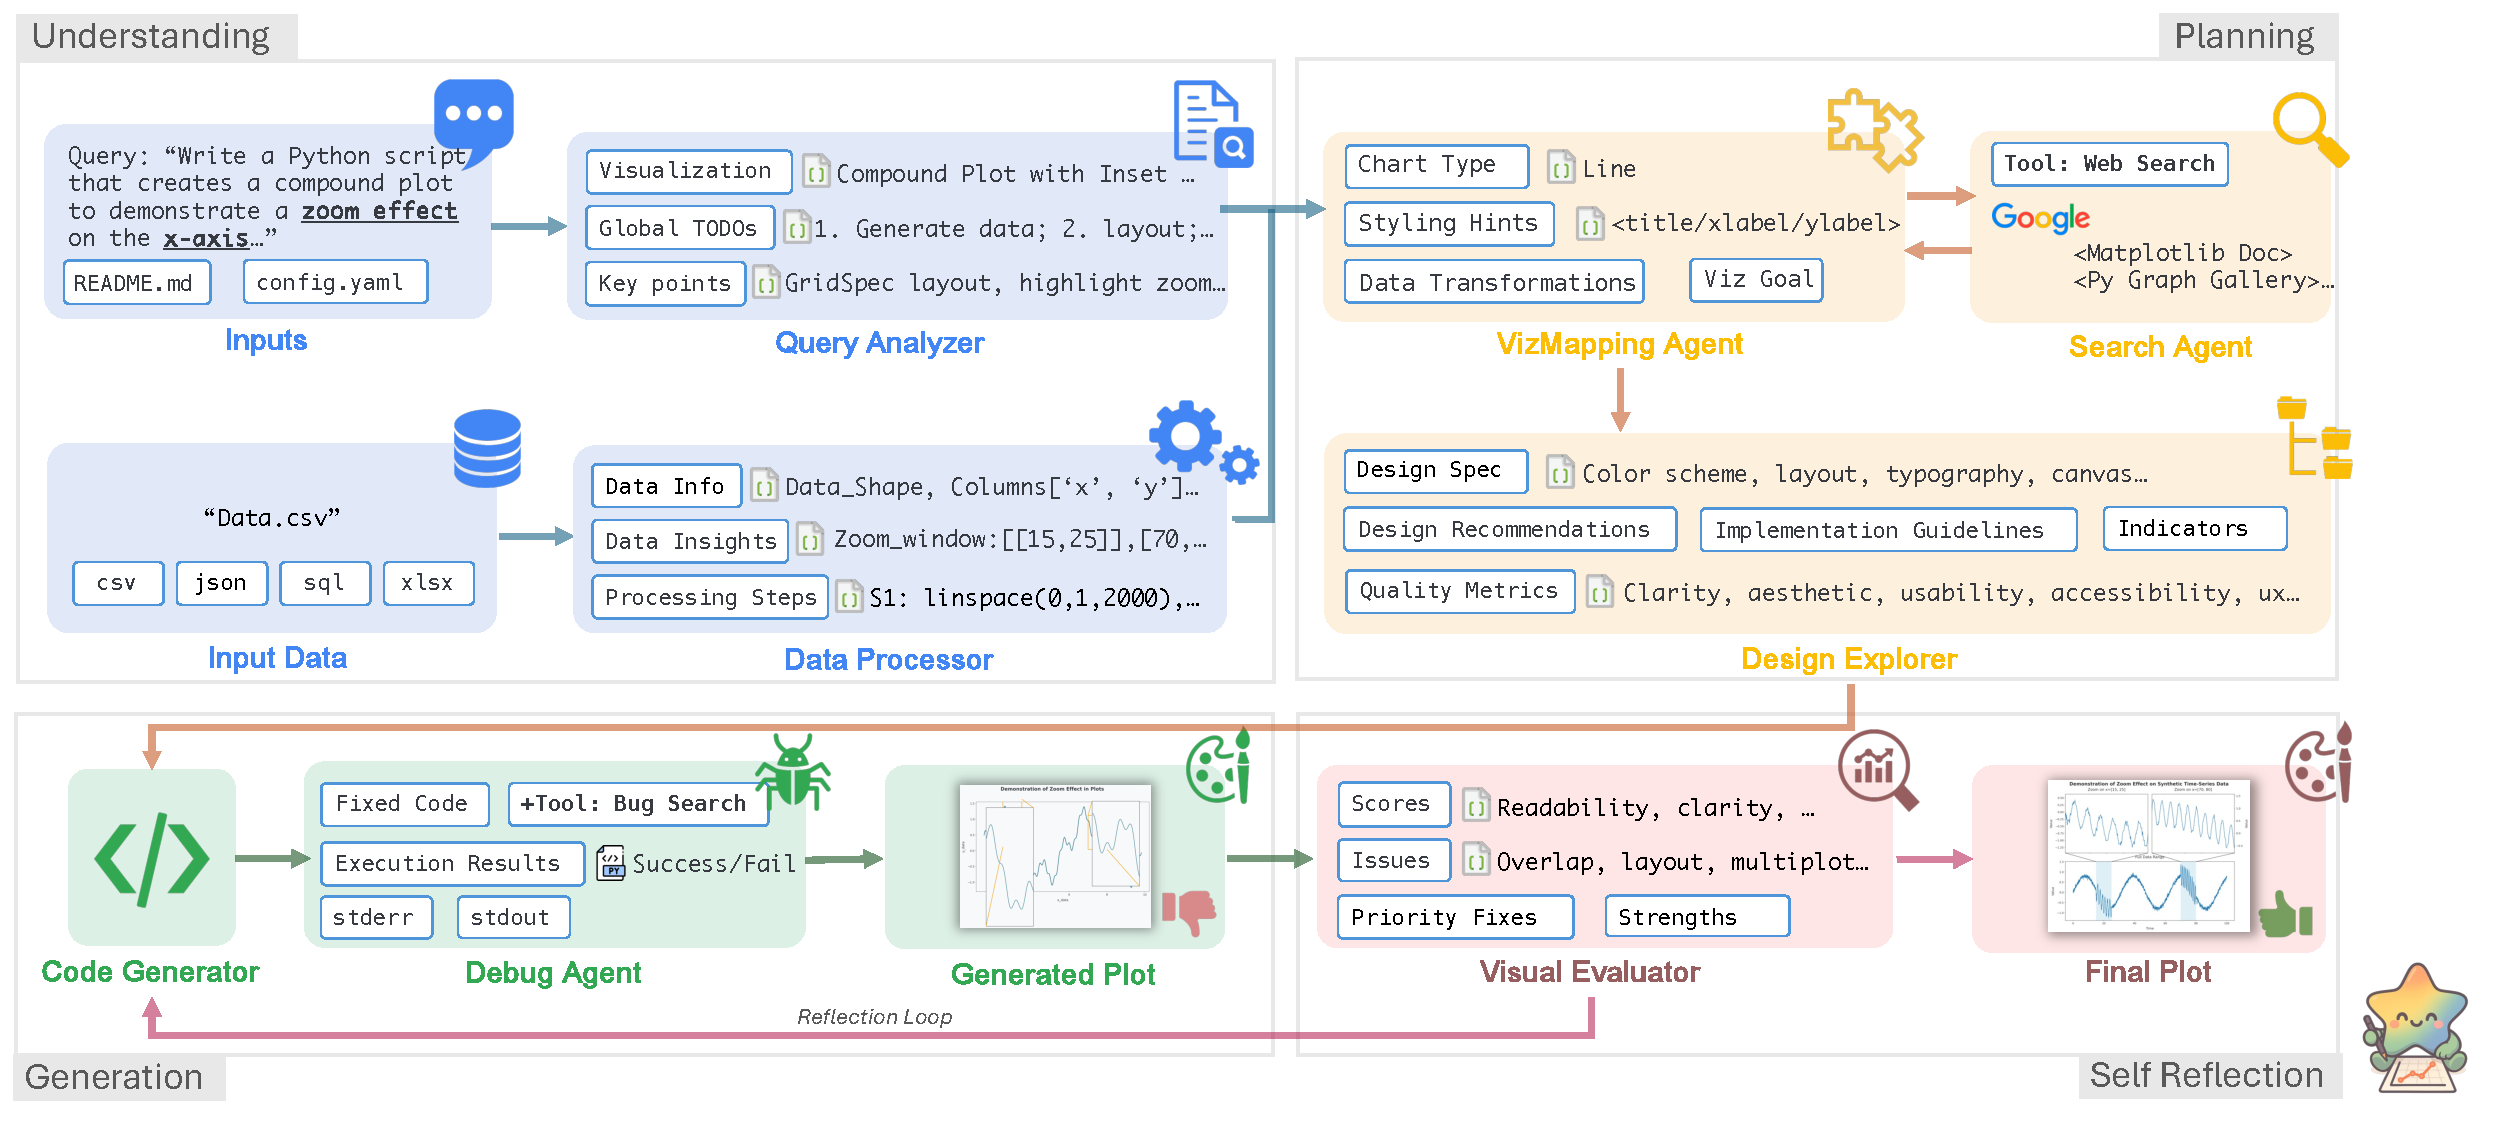
\includegraphics[width=\linewidth]{figures/workflow_logo.pdf}
    \caption{Overview of the \methodname{} framework for agentic data visualization. The workflow decomposes natural language queries into modular phases: \textbf{\textcolor{StarIndigo}{Understanding}} (query intent and data metadata extraction), \textbf{\textcolor{StarYellow}{Planning}} (example code search, visual mappings, and design optimization), \textbf{\textcolor{StarTeal}{Generation}} (code generation and debugging), and \textbf{\textcolor{StarCoral}{Self-Reflection}} (quality evaluation with feedback loops for self-reflection refinement). }
    \label{fig:main}
\vspace{-10pt}
\end{figure}


\subsection{The Collaborative Multi-Agent Paradigm}

Conventional visualization systems, whether rule-based or LLM-driven~\citep{khan2025evaluating,zhu2025open,Hutchinson2024LLMAssistedVA,shin2025visualizationary}, typically treat visualization as a monolithic, single-pass process of parsing a query, ingesting data, and generating code.
This leads to unstable performance on complex queries involving multi-file datasets, ambiguous requirements, or iterative refinements. We reframe visualization as a collaborative problem-solving endeavor. Our approach employs a team of specialized LLM agents, each with a distinct professional persona, that uses structured communication and quality-driven feedback loops to decompose queries, process data, and iteratively refine outputs.

Inspired by multi-agent systems in software engineering~\citep{Yang2024SWEagentAI} and interactive reasoning~\citep{Yao2022ReActSR}, this paradigm leverages the emergent capabilities of LLMs to simulate division of labor. Each agent is designed to focus on well-defined expertise area, such as metadata extraction or code debugging, while communicating via a shared state to adapt dynamically. This not only mitigates token limits by avoiding raw data ingestion but also enhances robustness through reflection and error correction, mirroring how data analysts collaborate to refine insights.
Key principles guiding this approach include:

\textbf{\textcolor{StarIndigo}{Specialization for Depth:}} Assign agents to distinct roles (e.g., planning vs. execution) to deepen reasoning without overwhelming a single model.

\textbf{\textcolor{StarIndigo}{Metadata-Centric Preprocessing:}} Summarize data structures upfront to inform downstream decisions, bypassing the need for full data loading.

\textbf{\textcolor{StarIndigo}{Iterative Reflection:}} Incorporate human-like evaluation of outputs (e.g., via image analysis) to detect and correct issues like visual clutter or factual inaccuracies.

\textbf{\textcolor{StarIndigo}{Modular Extensibility:}} Design agents as interchangeable modules, allowing integration of new tools or models for evolving tasks.


By unifying query understanding, data handling, code generation, and quality assurance into a self-reflection workflow, this approach transforms visualization from isolated code generation into a resilient, adaptive process. We demonstrate its efficacy through \methodname{}, which operationalizes these principles for real-world benchmarks.

\subsection{\methodname{}: Collaborative Data Visualization Agents}

\methodname{} instantiates the collaborative paradigm as a multi-agent system that takes a natural language query and data files as input, producing a refined visualization as output. Figure~\ref{fig:main} provides a high-level overview and Table~\ref{tab:agent_roles} summarizes the inputs and outputs of different agents in the workflow. 
Full agents prompts and I/O are shown in Appendix~\ref{appendix:prompts}.

% \begin{table}[htbp]
% \centering
% \caption{The inputs and outputs of different agents in the proposed \methodname{} framework.}
% \label{tab:agent_roles}
% \footnotesize
% \begin{tabular}{p{2.2cm}|p{4cm}|p{9cm}}
% \hline
% \textbf{Agent Name} & \textbf{Inputs} & \textbf{Outputs} \\ \hline
% Query Analyzer & Query, meta\_data (e.g., \io{README.md}) & Query analyzer results including visualization types, key points for plotting, a global TODO list. \\ \hline
% Data Processor & Data inputs & Data processor results including data information (e.g., \io{shapes}, \io{columns}), data insights (e.g., \io{aggregations\_needed}), processing steps, visualization hints. \\ \hline
% VizMapping Agent & Query, query analyzer, data processor results & Chart types, styling hints, data transformations (e.g., \io{aggregations}, \io{filters}), visualization goals. \\ \hline
% Search Agent & Visualization types, chart types & Code examples. \\ \hline
% Design Explorer & Query analyzer results, data processor results & Design explorer results including design specifics (e.g., \io{color\_scheme}, \io{layout}), implementation guidelines, quality metrics, design recommendations, alternative designs, and success indicators. \\ \hline
% Code Generator & Design explorer results, data processor results, search agent results, (self-reflection) visual evaluator results & Code generator results including generated code, code quality score, dependencies, and documentation. \\ \hline
% Debug Agent & Code generator results & Debugging results including standard outputs/errors, web-searched debug suggestions, fixed code, execution results and the output file. \\ \hline
% Visual Evaluator & Output file, query, query analyzer results, data processor results & Scores (e.g., \io{overall\_score}, \io{readability}), strengths, issues, priority fixes, code modifications, and recommendations. \\ \hline
% \end{tabular}
% \end{table}


\begin{table}[htbp]
\centering
\caption{Inputs and outputs of different agents in the proposed \methodname{} framework.}
\label{tab:agent_roles}
\footnotesize
\setlength{\tabcolsep}{5pt}
\renewcommand{\arraystretch}{1.3}
\rowcolors{2}{gray!5}{white}
\begin{tabular}{p{2.8cm} p{4.5cm} p{8.2cm}}
\toprule
\rowcolor{gray!20}
\textbf{Agent Name} & \textbf{Inputs} & \textbf{Outputs} \\
\midrule
Query Analyzer & Query; meta\_data (e.g., \io{README.md}) & Visualization types; key points for plotting; global TODO list. \\
Data Processor & Data inputs & Data info (e.g., \io{shapes}, \io{columns}); insights (e.g., \io{aggregations\_needed}); processing steps; visualization hints. \\
VizMapping Agent & Query; query analyzer; data processor results & Chart types; styling hints; transformations (e.g., \io{aggregations}, \io{filters}); visualization goals. \\
Search Agent & Visualization types; chart types & Code examples. \\
Design Explorer & Query analyzer; data processor results & Design specifics (e.g., \io{color\_scheme}, \io{layout}); implementation guidelines; quality metrics; design recommendations; alternatives; success indicators. \\
Code Generator & Design explorer; data processor; search agent; visual evaluator & Generated code; code quality score; dependencies; documentation. \\
Debug Agent & Code generator results & Debugging outputs/errors; web-searched fixes; corrected code; execution results; output file. \\
Visual Evaluator & Output file; query; analyzer; processor results & Scores (e.g., \io{overall\_score}, \io{readability}); strengths; issues; priority fixes; modifications; recommendations. \\
\bottomrule
\end{tabular}
\end{table}


The workflow proceeds as follows, with iterative refinement triggered by quality assessments: Query Analyzer interprets the query (e.g., \textit{``Plot sales trends by region''}) to extract intent, decomposes it into a global TODO list (e.g., data filtering, aggregation, chart selection), and generates guidelines for downstream agents. Data Processor extracts metadata summaries (schemas, statistics, patterns) from data files using lightweight tools like pandas, avoiding token limits while identifying insights and potential transformations. 
VizMapping maps query semantics to visualization primitives, selects appropriate chart types (e.g., line chart for trends), defines data-to-visual bindings, and validates compatibility based on metadata. This agent ensures insightful outputs that adapt to data complexities without raw ingestion.
Search Agent (as a tool) retrieves relevant code examples from plotting libraries (e.g., Matplotlib) to inspire generation, formulates search queries and ranks results by relevance. Design Explorer generates content and aesthetic concepts, optimizes elements like colors and layout, and evaluates designs for user experience. Code Generator synthesizes executable Python code integrating specifications, ensuring best practices and documentation. Debug Agent executes code with timeouts, diagnoses errors (e.g., via searched solutions), applies fixes (potentially via searched solutions), and outputs results like visualization images. Visual Evaluator assesses the output image across multi-dimensional quality metrics (clarity, accuracy, aesthetics, layout, correctness), verifying TODO completion and suggesting refinements.

Agents exchange structured messages through a shared memory buffer, propagating context (e.g., metadata informs planning, plans guide code). Feedback loops trigger self-reflection: If quality scores (from evaluation) are below thresholds, issues are routed back to upstream agents (e.g., low aesthetics back to the Design Explorer). The system halts when quality converges or reflection limits are reached.
\methodname{}'s modular design promotes scalability, agents can be parallelized or extended (e.g., scientific plotting), and self-reflection through quality-driven halting (e.g., stop if scores exceed thresholds). In experiments (Section~\ref{sec:exp}), this yields substantial gains over baselines, validating the value of this agentic approach in visualization automation.



